\chapter{微服务架构与跨数据链协议互操作系统设计}

本章基于MIL-STD-6016战术数据链信息标准,设计并实现微服务架构的跨协议互操作系统。系统架构采用四层分层设计,通过微服务模块化实现多标准信息模型的自动导入、语义对齐与协议转换。本章依次阐述系统总体架构、微服务实现、数据模型设计、跨协议互操作架构以及自动化导入系统。

\section{系统总体架构设计}

\subsection{设计目标与总体思路}

系统以MIL-STD-6016战术数据链信息标准为核心,采用微服务架构构建跨协议互操作平台。设计目标包括:多源标准语义互操作、模块化弹性部署、自动化数据处理。

多源标准语义互操作要求系统支持MIL-STD-6016、STANAG 5516、MIL-STD-6020、MQTT、MAVLink等协议的语义对齐。通过统一语义模型和概念映射机制,实现跨标准数据的准确转换,保障不同协议间的语义一致性。

模块化弹性部署通过微服务架构将复杂系统拆分为独立服务模块。每个服务专注特定业务功能,支持独立开发、测试、部署和扩展,提高系统的可维护性、可扩展性和容错能力。

自动化数据处理实现标准化文档的自动识别、结构化提取和协议转换。系统减少人工干预,提高数据处理效率和准确性,支持战术数据链信息处理的自动化。

\subsection{微服务架构理念与原则}

系统采用"高内聚、低耦合、自治服务"的设计理念,遵循四个核心原则:服务拆分、服务治理、数据管理、通信机制。

服务划分基于业务领域,保证每个微服务的独立性和单一职责。微服务负责业务中的某一部分,界限清晰,彼此间通过明确定义的接口(API)进行交互,避免紧耦合依赖。

服务治理包括注册发现、配置中心、监控系统、熔断器。服务注册中心自动发现结合负载均衡,配置中心统一管理与热加载,监控系统健康监控的同时也进行统计分析。

数据管理采用数据库解耦及分布式事务一致性保证,每个微服务都有自己的数据库,采用事件驱动分布式事务一致性保证,事件驱动分布式事务一致性保证的Saga模式,数据解耦和避免单点故障。

通信机制结合了通信+同步(REST/gRPC)+异步(消息队列)。实时性高的场景采用同步通信,大批量处理、事件通知采用异步通信,通信效率、系统性能。

\subsection{架构总体分层}

系统整体采用四层分层架构,如图\ref{fig:system_architecture}所示:

\begin{figure}[H]
    \centering
    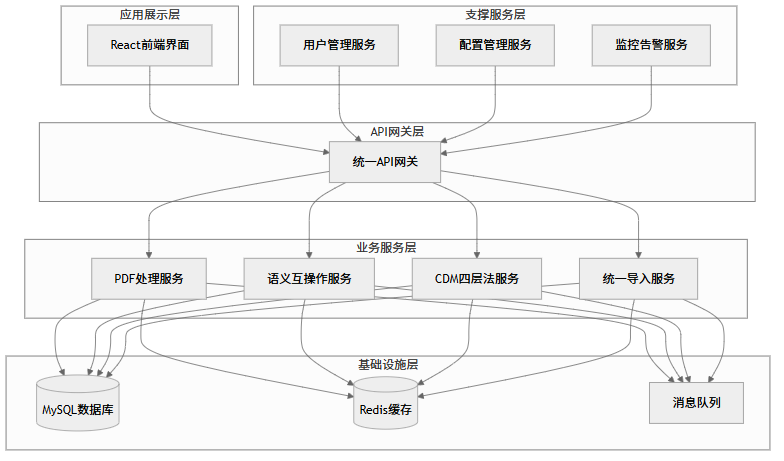
\includegraphics[width=0.9\textwidth]{chapters/fig-0/system_architecture_simple.png}
    \caption{系统总体架构分层图}
    \label{fig:system_architecture}
\end{figure}

API网关层提供系统统一接口,进行路由转发、认证鉴权、权限控制、限流熔断以及监控统计。外部的请求通过API网关层进行接收,对请求进行身份识别、鉴权、路由转发、聚合响应,通过限流、熔断对后端服务进行防护。

业务服务层包含PDF解析、语义互操作、CDM四层法、统一导入等核心业务模块。每个服务作为独立业务单元,支持独立开发、测试和部署,体现微服务架构的模块化设计理念。

支撑服务层包括用户认证、配置管理、监控告警、文件日志等系统支撑。支撑服务层是系统的核心,是整个系统运行的基础,包括用户认证、配置管理、监控告警、文件日志等功能。

基础设施层包含服务注册发现(Consul/Kubernetes)、消息队列(RabbitMQ/Redis)、数据库与缓存集群等核心组件。该层实现服务发现、消息传递、数据存储和缓存等基础功能,为微服务架构提供技术支撑。

\section{微服务架构设计}


\subsection{微服务模块划分与职责}

系统共包含五类核心服务,每个服务都有明确的职责和边界,如表\ref{table:microservices}所示:

\begin{table}[H]
    \caption{微服务模块划分与职责}
    \label{table:microservices}
    \centering
    \begin{tabular}{ll}
        \toprule
        \textbf{模块} & \textbf{核心职责} \\
        \midrule
        pdf-service & 自动化标准文档解析与结构化导入 \\
        semantic-service & 跨标准语义分析与字段映射 \\
        cdm-service & CDM四层语义互操作(语义层/映射层/校验层/运行层) \\
        import-service & 多格式文件识别、清洗与批量导入 \\
        api-gateway & 统一接口访问控制、负载均衡、服务监控 \\
        \bottomrule
    \end{tabular}
\end{table}

(1)pdf-service:负责自动化标准文档解析与结构化导入。服务处理MIL-STD-6016、STANAG 5516等标准文档,自动提取消息定义、字段信息和约束条件,转换为结构化数据格式。

(2)semantic-service:实现跨标准语义分析与字段映射。服务提供语义分析引擎,识别不同标准中的语义概念,建立概念间映射关系,支持人工标注和规则学习。

(3)cdm-service:实现CDM四层语义互操作。服务基于Common Data Model四层架构,提供语义层、映射层、校验层和运行层的完整实现,支持不同协议间的语义级转换。

(4)import-service:负责多格式文件识别、清洗与批量导入。服务支持PDF、Excel、XML、JSON等多种格式的文件处理,提供格式自动识别、数据清洗和批量导入功能。

(5)api-gateway:提供统一接口访问控制、负载均衡、服务监控。服务作为系统统一入口,负责请求路由、身份验证、权限控制、限流熔断和监控统计。

\subsection{微服务通信机制}

根据微服务架构的分布式特性,设计多种通信方式满足不同场景和通信安全需求。同步通信设计采用REST API、gRPC、GraphQL三类协议,REST API提供统一的标准化HTTP接口和简单的CRUD接口, gRPC提供高性能的内部服务调用接口, GraphQL提供复杂数据查询的灵活性。异步通信设计采用RabbitMQ提供消息和事件通知服务,确保系统关键业务数据的准确到达。服务发现设计采用Consul注册发现、Kubernetes DNS提供服务发现和负载均衡,实现系统服务启动时自动注册到服务发现中心,其他服务以服务名调用,松耦合实现服务通信。为确保通信安全,各服务之间通信均采用TLS通信,采用JWT令牌进行认证,建立安全屏障。

\subsection{容错与弹性设计}

考虑到分布式系统的复杂性和不确定性,系统提供了完善的容错和弹性策略。熔断器策略作为第一道屏障,当服务调用失败率达到预设值时,启动熔断器,进行服务熔断、服务快失败、服务故障隔离,防止故障的级联。重试策略基于指数退避算法和智能重试算法,对临时性故障自动重试,防止故障服务的过多接入。降级策略考虑当前系统负载过高或部分服务不可用时,自动降低服务复杂度,降级至简单模式,提供核心可用服务。自动伸缩策略使用 Kubernetes HPA 对服务根据 CPU、内存资源占比等指标自动扩充或缩减服务实例数量,实现弹性伸缩。

\section{数据模型与数据库设计}

\subsection{设计目标与数据特征}

战术数据链信息标准数据库的复杂性和多样性特征决定了系统必须采用"标准化存储、语义扩展、互操作可追溯"的设计原则,构建支持多标准数据管理的核心能力体系。统一建模与版本化管理机制确保系统能够支持MIL-STD-6016、STANAG 5516、MIL-STD-6020等多个标准版本的数据存储,每个标准版本具有独立的版本标识和变更历史,保障不同标准版本数据的独立性和可追溯性。

字段级语义绑定与跨标准映射提供语义互操作能力基础,通过语义的跨标准映射,将数据库中的每字段与语义绑定,具有跨标准的字段级映射与转换支持,映射关系包含置信度、转换规则、版本,提供语义互操作的数据转换支持。此外,还支持高性能的查询与语义检索,支持标准版本、消息类型、语义概念等的查询,支持全文检索、模糊匹配等功能。
\subsection{核心实体与关系模型}

系统的核心数据模型如图\ref{fig:data_model}所示,主要包含以下核心表:

\begin{figure}[H]
    \centering
    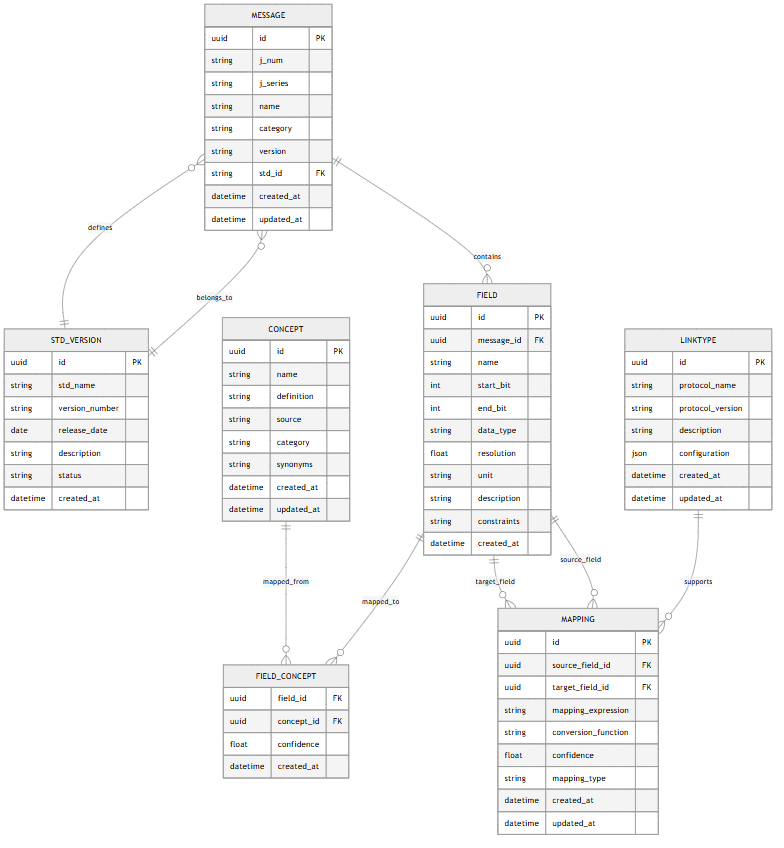
\includegraphics[width=0.9\textwidth]{chapters/fig-0/data_model.png}
    \caption{核心数据模型ER图}
    \label{fig:data_model}
\end{figure}

(1)MESSAGE表:存储消息元信息,包含消息编号、名称、类别、版本等基本信息。该表是系统核心表之一,每个消息具有唯一标识符和版本信息,为战术数据链消息的标准化管理提供数据基础。

(2)FIELD表:存储位段定义及约束信息,包含起始位、结束位、分辨率、取值域等详细信息。该表与MESSAGE表通过外键关联,支持一个消息包含多个字段的复杂结构。

(3)CONCEPT表:存储语义概念库,定义术语与来源信息,为语义互操作提供概念基础。该表支持概念的定义、分类和关系管理,构建完整的语义概念体系。

(4)MAPPING表:存储跨标准映射规则,包含表达式、转换函数、置信度等信息。该表支持不同标准间的字段映射和转换规则定义,为语义互操作提供精确的转换机制。

(5)STD\_VERSION表:存储标准版本管理信息,记录标准的版本号、发布日期、修订历史等关键信息。该表为多标准版本管理提供完整的版本控制机制。

(6)LINKTYPE表:存储协议类型定义与配置信息,支持不同数据链协议的配置和管理。该表为多协议支持提供灵活的配置机制。

\subsection{约束与索引设计}

数据库设计采用严格的约束和高效的索引策略,确保数据完整性和查询性能,构建了完善的数据管理机制。

主外键采用了 UUID 主键+业务唯一约束的设计。其中 UUID 主键全局唯一,避免了分布式环境下的主键冲突问题;业务唯一约束(MESSAGE(j\_num, std\_id))避免了业务逻辑的混乱。

完整性约束实现位段检查(start\_bit < end\_bit)、置信度范围(0–1)等多种约束机制。这些约束通过数据库的CHECK约束实现,在数据层面确保数据的有效性,防止无效数据的入库。

索引策略设计组合索引(std\_id, j\_series, j\_num)和全文索引(概念模糊检索)等多种索引类型。组合索引支持多条件查询,提升复杂查询的性能;全文索引支持语义概念的模糊检索。

性能优化采用分区表和缓存。大量数据的表采用分区减少查询量,水平和竖直相结合,提升性能;热点数据使用缓存,采用Redis来提升访问速度。

\subsection{微服务数据库分离与一致性}

各微服务采用独立的数据库设计,通过多种机制保证数据一致性,构建了完善的分布式数据管理体系。

数据库分离要求每个微服务拥有独立的数据库,避免数据耦合和单点故障问题。这种设计提高系统的可扩展性和容错能力,使得各个服务能够独立演进和部署。

一致性机制采用 Saga 模式以及事件驱动并发式机制组合的方式来实现最终一致性。Saga 模式将分布式事务切割成多个本地事务并通过补偿模式来确保数据一致性,解决分布式事务中数据一致性。

数据同步通过CDC(Change Data Capture)机制捕获变更事件,实现数据的实时同步。CDC机制精确捕获数据库的变更操作,将变更事件发送到消息队列,为数据同步提供可靠的技术保障。

跨服务使用消息队列实现跨服务数据同步。当服务有变更时,系统将变更后的消息放入消息队列,并通知其他需要变更的服务进行数据更新,完成松耦合的数据更新。

\section{跨数据链协议互操作架构设计}

\subsection{多协议支持体系}

系统支持多种数据链协议,包括MIL-STD-6016、MAVLink、MQTT、Link 16等,构建了四层互操作体系架构,如图\ref{fig:multi_protocol_support}所示:

\begin{figure}[H]
    \centering
    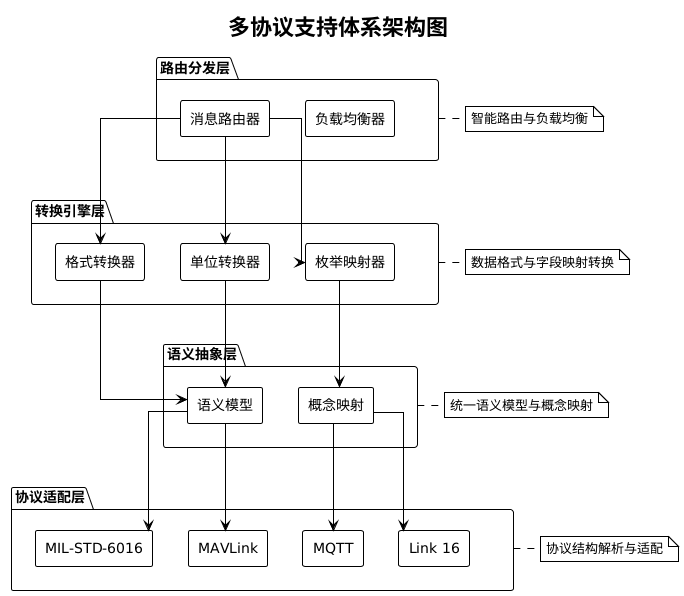
\includegraphics[width=0.8\textwidth]{chapters/fig-0/multi_protocol_support_simple.png}
    \caption{多协议支持体系架构图}
    \label{fig:multi_protocol_support}
\end{figure}

协议适配层是互操作体系结构的最底层,负责实现各个链路标准的结构解析适配,实现对各种协议消息格式进行解析处理,对字段信息进行解析,统一内表示,为上层处理提供一致接口。

语义抽象层建立统一的语义模型和概念映射机制,将各个协议中的概念映射到概念空间,采用语义建模的方式实现不同协议间的概念映射和语义理解,为协议间进行语义互操作奠定概念基础。

转换引擎层提供协议到协议的数据格式以及字段映射转换,如格式转换、单位转换、枚举转换等,提供丰富的转换规则配置方式以支持复杂的数据转换规则配置,转换规则灵活,支持复杂数据转换。

路由分发层负责消息的路由和负载均衡,将消息分发给正确的目标协议,实现负载均衡和故障转发。路由分发层采用智能路由算法进行消息路由,优化性能和可靠性。

\subsection{CDM四层法语义互操作模型}

基于"Common Data Model (CDM)"四层方法,系统实现了协议级语义对齐,构建了完整的语义互操作体系,如图\ref{fig:cdm_four_layer}所示:

\begin{figure}[H]
    \centering
    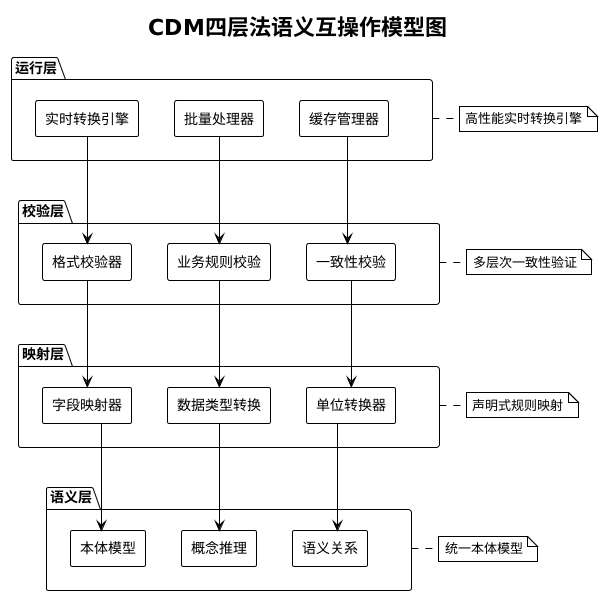
\includegraphics[width=0.6\textwidth,height=0.5\textheight]{chapters/fig-0/cdm_four_layer_simple.png}
    \caption{CDM四层法语义互操作模型图}
    \label{fig:cdm_four_layer}
\end{figure}

语义层是 CDM 的核心层,构建统一的本体模型及概念推理系统。通过本体技术建立统一的概念模型可以定义、分类和推理,使系统能够理解概念间的语义。

映射层采用声明式规则映射和YAML 配置化,通过 YAML 配置文件描述映射规则,便于规则变更与升级。映射规则包括字段映射、数据类型映射、单位映射等。

校验层提供多层次的一致性验证和金标准回归测试机制,包括格式校验、业务规则校验、一致性校验等多种校验方式。金标准回归测试确保转换结果的准确性,为语义互操作的质量提供可靠保障。

运行层提供高性能、高效率的实时转换引擎,采用高效的转换算法实时进行消息转换、批量处理,提供高效的实时转换缓存及优化,满足战术数据链的实时性高和性能高的要求。

\subsection{语义互操作系统组成}

系统包含四个核心组件,实现从概念级到消息级的自动语义互操作,构建了完整的语义互操作处理体系,如图\ref{fig:semantic_interop_system}所示:

\begin{figure}[H]
    \centering
    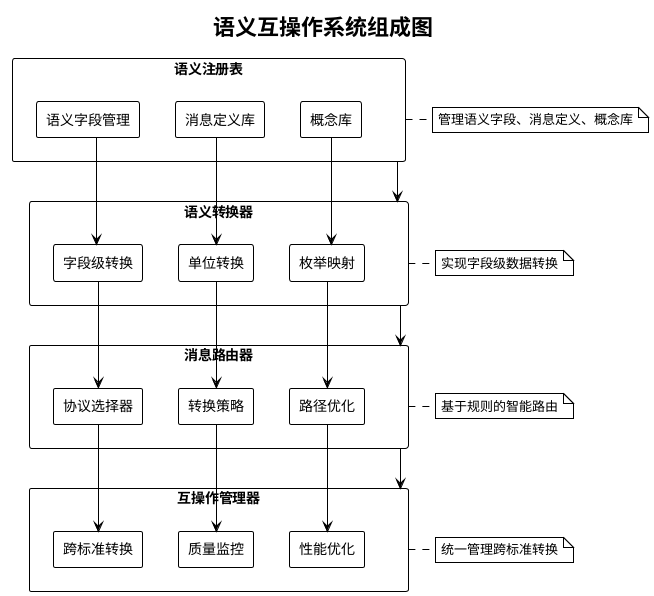
\includegraphics[width=0.8\textwidth]{chapters/fig-0/semantic_interop_system_simple.png}
    \caption{语义互操作系统组成图}
    \label{fig:semantic_interop_system}
\end{figure}

语义注册表是系统存放语义域、消息定义、概念库等系统基础信息的核心组件,提供语义信息的增删查改,支持语义概念版本控制,是进行语义信息交互操作的基础管理平台。

语义转换器实现字段级数据转换、单位转换、枚举映射等关键功能,该组件支持多种转换算法,包括数值转换、字符串转换、枚举映射等。通过灵活的转换规则配置,该组件能够处理复杂的跨协议数据转换需求。

消息路由器采用基于规则的智能路由模式,进行协议选择和转换策略的自动配置。消息路由器根据消息的类型、源协议、目的协议等,自动匹配最佳的转换策略,采用智能的算法来进行消息路由。

互操作管理器集成各种跨标准互操作转换、质量管控、性能调优等管控管理功能,此部件提供统计、错误管控、评分等转换监控与管理功能,通过对转换管理,确保了语义互操作运行的稳定高效。

\subsection{数据一致性与冲突解决}

系统采用多种机制保证跨链路数据的一致性和冲突解决,构建了完善的数据质量管理体系。

一致性协议采用最终一致性协议与版本号优先策略相结合的方式。对于非关键数据,使用最终一致性协议,在保证系统性能的同时确保数据的最终一致性;对于关键数据,使用强一致性保证,确保数据的实时一致性。

冲突解决采用时间戳优先、版本号优先、人工仲裁等策略实现,在数据冲突的时候,调用预定义的策略,自动解决冲突,通过智能冲突检测、智能冲突解决等智能算法,将数据冲突的影响范围降低到最小;必要情况下调用人工仲裁,确保复杂冲突场景下的数据准确性。

数据校验支持格式校验、规则校验、完整性校验等多层次的校验机制,每一层转换过程均进行校验,保证数据不错误、不缺失,通过多层次的校验机制确保了错误不传播。

质量保障跨链路数据同步数据质量保障,通过持续不断地对数据转换的质量,也就是准确率、完整性、一致性等的监控。实时质量保障监控和告警,系统能够实时发现数据质量问题并给出解决方案。

\section{自动化信息标准导入架构设计}

\subsection{标准化导入流程}

自动化导入系统实现从PDF/Excel/XML等标准文档到数据库的全流程自动处理,如图\ref{fig:import_pipeline}所示:

\begin{figure}[H]
    \centering
    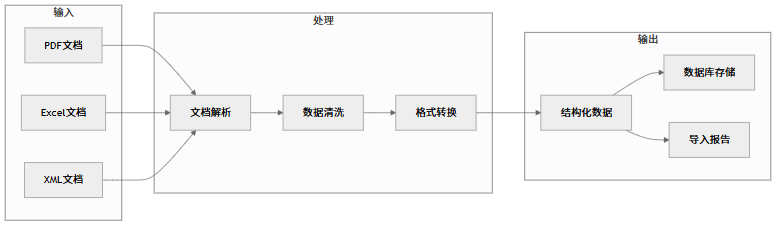
\includegraphics[height=0.5\textheight,keepaspectratio]{chapters/fig-0/import_pipeline_simple.png}
    \caption{自动化导入流程}
    \label{fig:import_pipeline}
\end{figure}

处理过程是文本导入-数据清洗-文本抽取-表格识别、字段分析、数据清洗、入库、形成校验报告等。每一步处理都经过检验和审核,确保了导入到系统中的数据完整、干净、准确。

文档解析阶段使用 OCR 技术和 PDF 分析库,从文档中提取文本、表格。扫描文档使用 Tesseract OCR,识别文字,多语言文本识别;文本类 PDF 直接提取文本,多种解析技术,确保不同类型文档解析正确。

在结构化处理阶段,将提取出的文本信息进行结构化处理,将消息定义、内容字段、约束条件信息等通过规则匹配和机器学习算法进行识别,将非结构化的文档信息转化为结构化的、统一的数据结构。

在清洗数据阶段,对抽取出的数据进行清洗校验,包括:格式校验、完整性校验、一致性校验等校验。将校验出的问题写入日志错误文件,以便后续处理和分析。

导入存储将清洗完成的数据导入入库并生成导入报告,导入报告包括导入成功的记录数,导入失败的记录数,以及具体的错误信息等统计指标,为整个导入过程提供详尽的数据以便分析导入的质量和出现的问题追根溯源。

\subsection{关键技术与工具链}

系统采用多种先进的技术和工具,确保导入过程的准确性和效率,构建了完整的技术支撑体系。

文档解析工具主要有:PyMuPDF、pdfplumber、Camelot、TesseractOCR等等,PyMuPDF是一个十分先进的分析文档的软件,pdplumber软件是抽取表格工具,Camelot软件是抽取准确表格工具,TesseractOCR是文字识别工具,多种工具结合使用,确保正确分析不同类型的文件。

结构化导入采用Pandas + SQLAlchemy + MySQL技术架构。Pandas海量数据计算分析;SQLALCHEMY负责ORM的支持,方便数据库操作;MySQL可靠地进行了数据存储,保持数据的一致性、安全性。

格式识别使用MIME 检测,采用格式识别与规则匹配相结合的格式识别方式。MIME 检测速度较快,识别文件的格式,为后续对文件处理提供基本信息;规则匹配提供精确的格式识别与内容识别,通过智能识别算法,对不同的格式文档进行精准的识别。

校验机制实现字段重叠、位长一致、枚举合法等校验功能。自动对数据中存在的问题进行检查,并提示修复建议,通过智能校验机制,保证导入数据质量。


\subsection{数据清洗与质量保证}

系统提供完善的数据清洗和质量保证机制,构建了全方位的数据质量管理体系。

清洗算法支持空值、重复、一致性等检测。系统自动处理缺失值、重复值、错误值等常见错误,通过应用清洗算法对数据进行智能清洗,实现数据清洗。

质量指标监控系统数据完整性、语义保留度、转化率等。这些指标可以综合评估数据的质量,为数据质量的优化提供参考,数据质量监控系统能帮助系统及时发现并处理数据质量问题。

验证机制提供格式验证、业务规则验证、一致性验证等多层次的验证机制,不同的层次具有不同的验证机制,并具有对应的错误处理,多层次验证确保了数据的一致性和准确性。

错误处置能够完成异常记录、自动修正、人工校验等功能,系统大部分问题能够实现自动处理,仅对于复杂问题需要部分人工干预,从而通过智能的差错处理减少最大可能的数据质量问题。

\section{微服务通信与运行保障设计}

\subsection{服务通信与安全}

系统采用多种通信模式和安全机制,确保服务间的可靠通信,构建了完善的通信安全保障体系。

同步通信使用REST API、gRPC、GraphQL等多个协议。Rest API,用于简单的增删改查并使用统一的HTTP接口;gRPC,用于高性能的内部通信,二进制协议效率高;GraphQL则主要用于复杂的数据查询,提供灵活的数据获取能力。

异步通信采用了RabbitMQ、Redis Pub/Sub的技术组合。采用RabbitMQ提供可靠的消息传递和事务支持以确保关键业务数据的可靠传输;而Redis Pub/Sub提供了高性能的实时通知以及支持轻量级消息传递,从而创建了同步与异步相结合的通信机制。

服务发现通过Consul + Kubernetes DNS实现服务的自动发现和负载均衡。服务启动时自动注册到服务发现中心,其他服务通过服务名进行调用,实现服务间的松耦合通信,提高系统的可维护性和可扩展性。

通信安全使用TLS双向认证、服务间认证通信安全,服务间通信均采用TLS加密通信、JWT令牌认证,构建多层次安全体系。

\subsection{分布式数据管理与灾备}

系统采用分布式数据管理策略,确保数据的安全性和可用性,构建了完善的数据保护体系。

数据分离实现数据分离、数据所有权隔离,由于微服务各自独立存储数据,不会造成数据的耦合、单一失效,使系统可扩展性、容错性得到极大地提高,为微服务架构的灵活性提供了数据基础。

一致性保证采用Saga与溯源的方式,达成一致的一致性结果。Saga模式是将复杂分布式事务切分为多个本地事务,并通过补偿事务的方式保证一致性结果,解决分布式事务中数据的一致性问题。

灾备机制实现多区域备份与灾难恢复机制。系统支持跨区域的数据备份和灾难恢复,确保在重大故障情况下的数据安全,通过完善的灾备体系,最大程度地降低数据丢失的风险。

数据同步支持实时同步、批量同步、增量同步等多种数据同步模式。系统能够根据数据的重要程度、实时性要求等智能选择数据同步方式。

\subsection{配置与治理体系}

系统提供完备的配置管理和服务治理能力,形成完整的系统治理体系。

配置管理提供集中配置与隔离(Consul + Configmap)。系统配置集中存储在配置中心,动态更新和隔离,通过统一的配置管理提供系统配置一致性、易维护能力,提供多环境部署灵活配置的能力。

监控体系提供全链路监控(Prometheus + Grafana + Jaeger)能力。Prometheus负责指标收集,提供全面的性能监控数据;Grafana提供可视化展示,支持丰富的图表和仪表板;Jaeger提供分布式链路追踪,实现完整的系统监控体系。

日志管理实现结构化日志与追踪链路功能。所有日志都采用结构化格式,支持日志聚合、搜索和分析,通过统一的日志管理,为系统运维和问题排查提供强有力的支撑。

服务治理提供健康检查、故障检查、负载均衡等服务的治理功能,系统自动进行服务健康检查、服务转移故障、负载均衡、智能服务治理、保障系统稳定、高可用。

\subsection{容错与弹性设计}

系统采用多种容错和弹性设计机制,确保在异常情况下的服务可用性,构建了完善的故障处理体系。

容错机制容错机制保障熔断、重试、降级机制保障系统容错服务可用当服务调用失败率达到阈值时系统自动熔断,避免系统断链;临时性问题自动重启;系统能力超负荷时,系统自动降级,保障核心服务可用。

弹性伸缩使用 Kubernetes HPA 实现弹性伸缩、资源弹性分配。系统根据 CPU 占用率、内存占用率和自定义指标,自动调整服务副本数量,动态分配资源,使系统保持高效。

故障恢复提供自动恢复、手动干预、数据修复等完整功能。系统能够自动处理大部分故障,对于复杂故障提供人工干预机制,通过智能化的故障处理,最大程度地减少故障对系统的影响。

性能保障确保响应时间保证、吞吐量稳定、故障恢复能力。系统通过多种优化技术,提供高性能和稳定的服务,满足战术数据链对系统性能和可靠性的严格要求。
